\documentclass{beamer}
\usetheme{Madrid}
\usepackage[T1]{fontenc}
\usepackage{mathpazo}
\usepackage{graphicx}
\usepackage{booktabs}
\usepackage{tikz}
\usetikzlibrary{positioning,arrows.meta,shapes.geometric,fit,backgrounds,calc}
\definecolor{cetnavy}{RGB}{10,26,63}
\definecolor{cetlight}{RGB}{225,231,242}
\setbeamercolor{structure}{fg=cetnavy}
\setbeamercolor{frametitle}{bg=cetnavy,fg=white}
\setbeamercolor{title}{bg=cetnavy,fg=white}
\setbeamertemplate{navigation symbols}{}
% =====================================================================
%  EDIT YOUR DETAILS HERE — this ONE file feeds every abstract & deck.
%  (Change a value, recompile; all 36 documents update.)
% =====================================================================
\newcommand{\seminarName}{Aflah Muhammed P}      % <-- your full name (guessed from your email; please verify)
\newcommand{\seminarRoll}{TVE00CS000}            % <-- your university register/roll number
\newcommand{\seminarClassRoll}{00}               % <-- your class roll no (the short one)
\newcommand{\seminarGuide}{Prof.\ <Guide Name>}  % <-- your guide
\newcommand{\seminarDept}{Department of Computer Science and Engineering}
\newcommand{\seminarCollege}{College of Engineering Trivandrum}
\newcommand{\seminarShortCollege}{CET}           % shown in the slide footer, e.g. "Aflah Muhammed P (CET)"
\newcommand{\seminarShortTitle}{B.Tech Seminar}  % middle of the slide footer
\newcommand{\seminarDate}{July 31, 2026}
% ---------------------------------------------------------------------
% Optional: put a logo image named  cet_logo.png  in this folder and it
% will appear on every title slide automatically. If absent, it is skipped.
% =====================================================================

\title[\seminarShortTitle]{CaMeL: Defeating Prompt Injection by Design}
\author[\seminarName\ (\seminarShortCollege)]{\seminarName \\ \seminarRoll \\ Roll No: \seminarClassRoll \\ Guide: \seminarGuide}
\institute[\seminarShortCollege]{\seminarDept \\ \seminarCollege}
\date{\seminarDate}
\titlegraphic{\IfFileExists{cet_logo.png}{\includegraphics[height=1.1cm]{cet_logo.png}}{}}
\begin{document}
\begin{frame}\titlepage\end{frame}
\begin{frame}{Table of Contents}\tableofcontents\end{frame}
\section{Introduction}
\begin{frame}{Agentic LLMs and a New Attack Surface}
\textbf{\textit{From chatbots to autonomous agents}}
\begin{itemize}
\item LLM agents call tools, read email, browse the web.
\item They must consume untrusted external content.
\item Trusted instructions and untrusted data share one context.
\item Attackers hide instructions inside that data.
\end{itemize}
\end{frame}

\begin{frame}{Why Prompt Injection Matters}
\begin{itemize}
\item Injected text can hijack the agent's actions.
\item Consequences: data theft, wrong recipients, unsafe tool calls.
\item Widely ranked as the top LLM security risk.
\item Filters and detectors are probabilistic and bypassable.
\end{itemize}
\end{frame}

\section{Literature Survey}
\begin{frame}{Prior Defenses Against Injection}
\begin{itemize}
\item Adversarial fine-tuning: hardens models, no guarantees.
\item Input detectors and classifiers for malicious text.
\item Prompt-level tricks: delimiters, spotlighting, instruction hierarchy.
\item Dual-LLM pattern (Willison): isolates untrusted text.
\item AgentDojo: benchmark for agent injection attacks and defenses.
\end{itemize}
\end{frame}

\begin{frame}{Gap in Existing Work}
\begin{itemize}
\item Most defenses rely on the model behaving correctly.
\item Adaptive attackers defeat probabilistic guardrails.
\item No guarantee on control or data flow.
\item CaMeL borrows ideas from systems security instead.
\end{itemize}
\end{frame}

\section{Motivation}
\begin{frame}{Security Should Not Rely on the Model}
\begin{itemize}
\item Defenses that ``mostly work'' still fail under attack.
\item A single successful injection can be catastrophic.
\item Treat the LLM as untrusted, not the enforcer.
\item Reuse proven ideas: capabilities and data provenance.
\end{itemize}
\end{frame}

\section{Problem Statement}
\begin{frame}{The Precise Problem}
\begin{itemize}
\item Untrusted data can alter agent control flow.
\item Agents can exfiltrate private data through tools.
\item Goal: stop injection without retraining the model.
\item Constraint: preserve usefulness on legitimate tasks.
\end{itemize}
\end{frame}

\section{Objectives}
\begin{frame}{Goals and Contributions}
\begin{itemize}
\item Separate control flow from untrusted data by design.
\item Track value provenance using capabilities.
\item Enforce security policies at every tool call.
\item Provide provable protection with minimal utility loss.
\end{itemize}
\end{frame}

\section{Methodology Overview}
\begin{frame}{Core Idea}
\textbf{\textit{Turn the trusted query into a program}}
\begin{itemize}
\item Trusted query becomes an explicit plan (code).
\item Plan encodes the control and data flow.
\item Untrusted data only fills values, never logic.
\item Interpreter guards each tool invocation.
\end{itemize}
\end{frame}

\begin{frame}{Methodology Overview}
\begin{center}
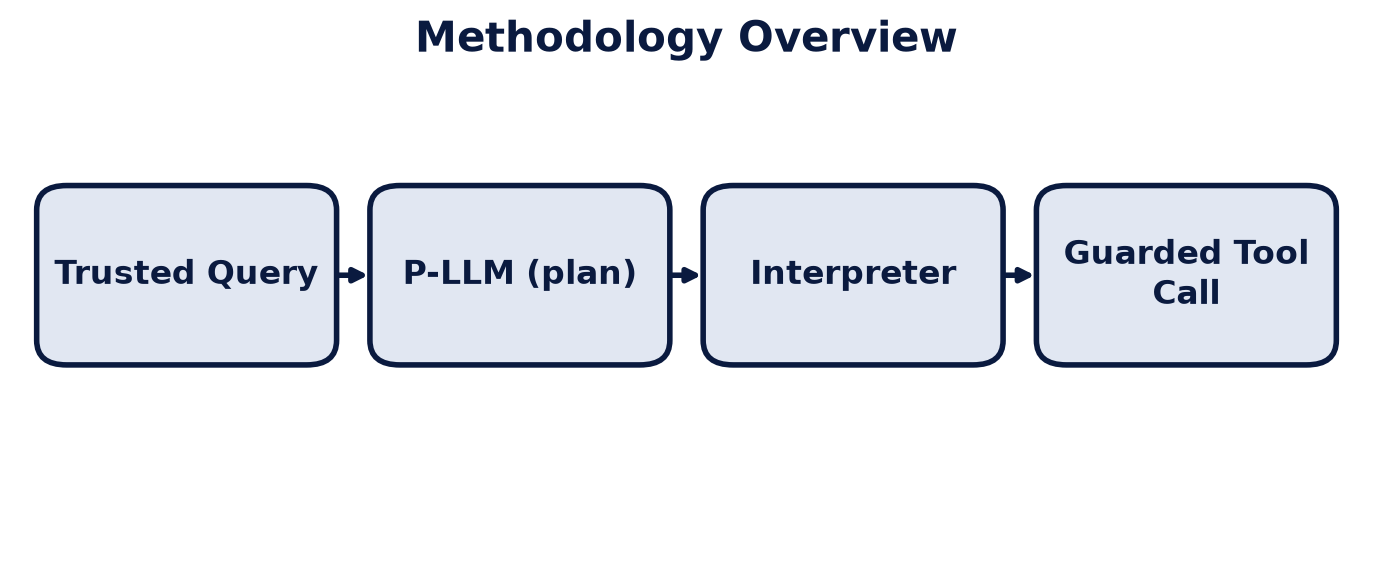
\includegraphics[width=0.9\textwidth,height=0.62\textheight,keepaspectratio]{images/camel_1.png}
\end{center}
\end{frame}

\section{System Architecture}
\begin{frame}{Two LLMs and One Interpreter}
\begin{itemize}
\item \textbf{P-LLM}: plans and writes code; sees only trusted query.
\item \textbf{Q-LLM}: parses untrusted data; has no tools.
\item \textbf{Interpreter}: runs the plan over restricted Python.
\item \textbf{Capabilities + policies}: gate each tool call.
\end{itemize}
\end{frame}

\begin{frame}{System Architecture}
\begin{center}
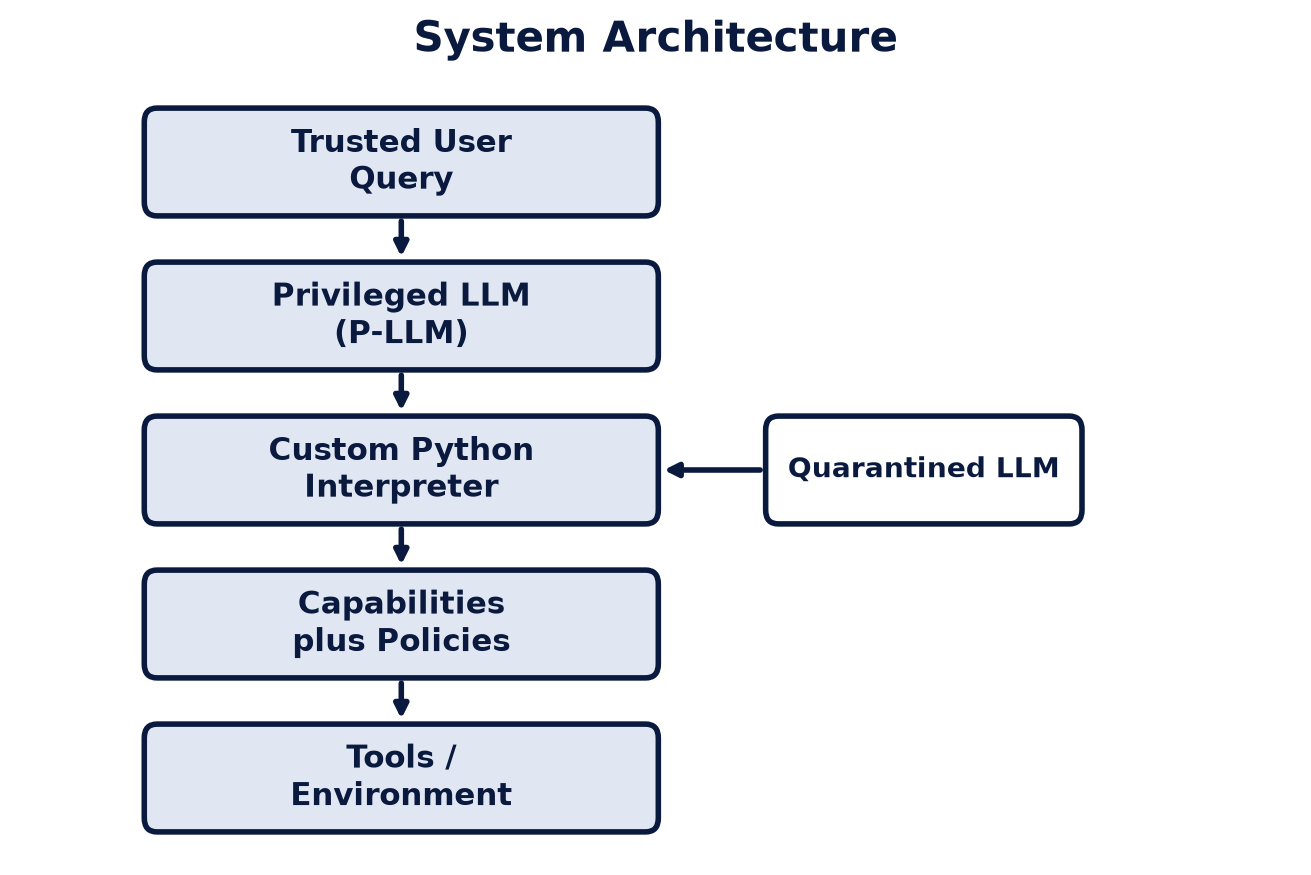
\includegraphics[width=0.9\textwidth,height=0.62\textheight,keepaspectratio]{images/camel_2.png}
\end{center}
\end{frame}

\section{Data Collection}
\begin{frame}{Evaluation Setup}
\textbf{\textit{Benchmark and metrics}}
\begin{itemize}
\item Evaluated on the AgentDojo agent-security suite.
\item Realistic tasks: email, banking, travel, workspace.
\item Injection attacks embedded in tool outputs.
\item Metrics: task utility and attack success rate.
\end{itemize}
\end{frame}

\section{Model Development}
\begin{frame}{How Capabilities Work}
\begin{itemize}
\item Every value carries provenance metadata (a capability).
\item Tags mark trusted versus untrusted origin.
\item Derived values inherit their sources' capabilities.
\item Policies read tags before allowing a tool call.
\end{itemize}
\end{frame}

\begin{frame}{Policy Enforcement at Tool Time}
\begin{center}
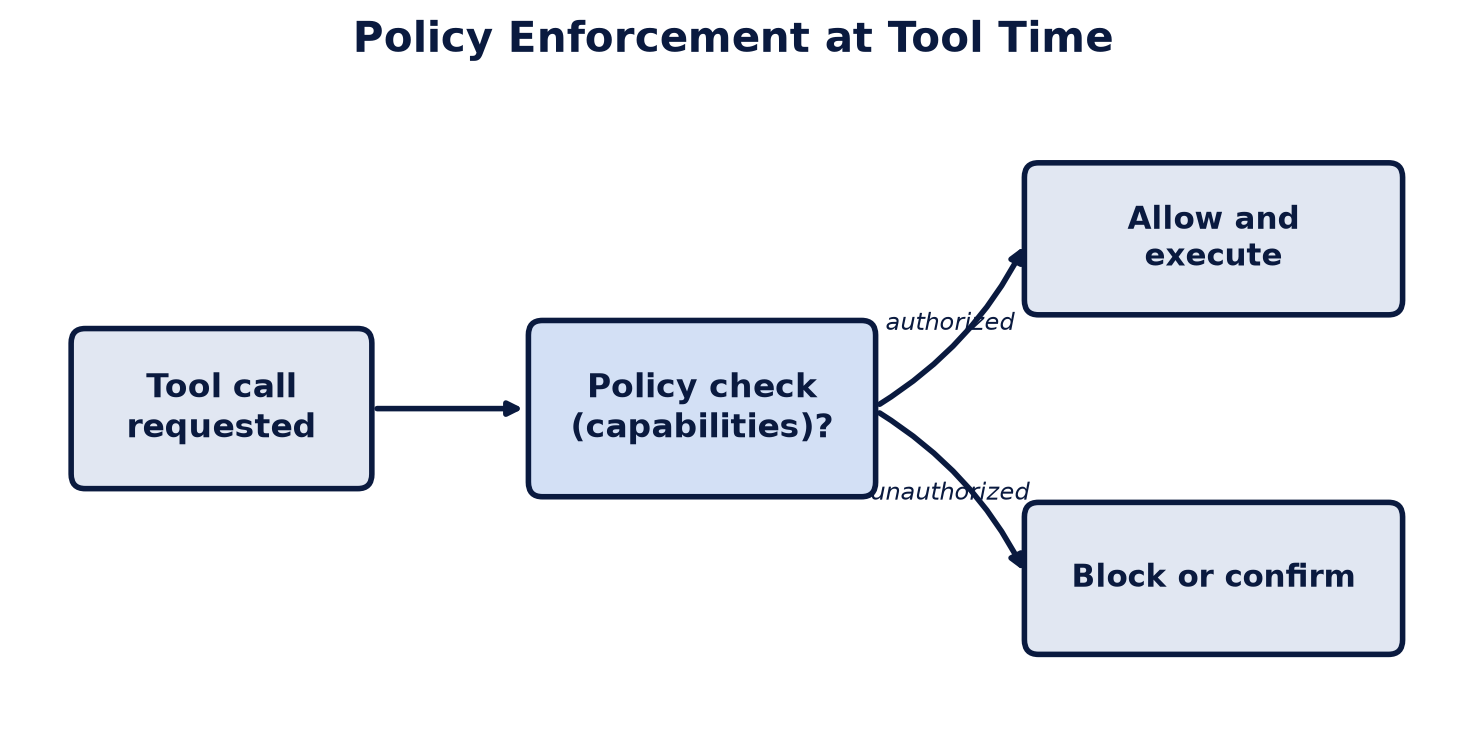
\includegraphics[width=0.9\textwidth,height=0.62\textheight,keepaspectratio]{images/camel_3.png}
\end{center}
\end{frame}

\section{Results}
\begin{frame}{AgentDojo Performance}
\begin{center}
\begin{tabular}{lcc}
\toprule
System & Task utility & Injection defense \\
\midrule
Undefended & $\sim$84\% & none \\
CaMeL & $\sim$77\% & provable \\
\bottomrule
\end{tabular}
\end{center}
\begin{itemize}
\item Provable security at a modest $\sim$7-point utility cost.
\item Exfiltration over unauthorized channels blocked by construction.
\item Protection holds even if the LLM is fooled.
\end{itemize}
\end{frame}

\section{Discussions}
\begin{frame}{Why It Works}
\begin{itemize}
\item Security comes from design, not model tuning.
\item Control and data flow are separated explicitly.
\item Untrusted data can influence values, never logic.
\item Trade-off: some flows require user confirmation.
\end{itemize}
\end{frame}

\section{Challenges}
\begin{frame}{Limitations}
\begin{itemize}
\item Users must codify and maintain security policies.
\item Confirmation prompts can cause user fatigue.
\item Q-LLM parsing errors may reduce utility.
\item Side channels are not fully eliminated.
\end{itemize}
\end{frame}

\section{Future Work}
\begin{frame}{Directions Ahead}
\begin{itemize}
\item Auto-generate policies from task context.
\item Reduce confirmation burden with safer defaults.
\item Extend the design to multi-agent systems.
\item Combine with formal verification of policies.
\end{itemize}
\end{frame}

\section{Conclusion}
\begin{frame}{Conclusion}
\begin{itemize}
\item Prompt injection is a design flaw, not a bug.
\item CaMeL isolates untrusted data by construction.
\item About 77\% of tasks solved with provable security.
\item A blueprint for building secure LLM agents.
\end{itemize}
\end{frame}

\section{References}
\begin{frame}{References}
\footnotesize
\begin{itemize}
\item E. Debenedetti, I. Shumailov, T. Fan, J. Hayes, N. Carlini, D. Fabian, C. Kern, C. Shi, A. Terzis, and F. Tram\`{e}r, ``Defeating Prompt Injections by Design,'' arXiv:2503.18813, 2025.
\item E. Debenedetti et al., ``AgentDojo: A Dynamic Environment to Evaluate Prompt Injection Attacks and Defenses for LLM Agents,'' NeurIPS Datasets \& Benchmarks, arXiv:2406.13352, 2024.
\item S. Willison, ``The Dual LLM pattern for building AI assistants that can resist prompt injection,'' simonwillison.net, 2023.
\end{itemize}
\end{frame}
\begin{frame}\vfill\centering{\Huge Thank You}\vfill\end{frame}
\end{document}
